\section{正弦交流的产生与有效值}

平面线圈在匀强磁场中绕垂直磁场的固定轴匀速转动，各匝面积为 $S$，匝数为 $N$。从法线与磁场重合的时刻计时，磁链 $\Psi=NBS\cos\omega t$，对复合函数求导时，先对相位 $\theta$ 求导，再乘 $\dot\theta=\omega$：
\[
 e=-\frac{\dd\Psi}{\dd t}
 =-NBS\frac{\dd\cos\theta}{\dd\theta}\frac{\dd\theta}{\dd t}
 =-NBS(-\sin\theta)\omega
 =NBS\omega\sin\omega t.
\]初始位置改变只改变相位，幅值仍为 $NBS\omega$。若转轴平行磁场，磁通不变，不会由这一转动产生相同的正弦电动势。

\fig{em6:generator-angle}{从转轴方向看线圈的投影；法向转角决定磁链，转轴垂直外磁场}{\begin{tikzpicture}

\foreach\y in {-.8,0,.8}{\draw[flow,blue](-2.3,\y)--(2.4,\y);}\node[blue]at(2.3,1.3){$\bm B$};
\draw[world,very thick](-.964,1.149)--(.964,-1.149);\draw[flow,red](0,0)--(1.532,1.286)node[above right]{$\bm n$};\draw[world](.8,0)arc(0:40:.8);\node at(1.15,.38){$\omega t$};\node at(0,0){$\odot$};\node[left]at(-.25,-.25){转轴};\node at(0,-1.9){线圈边视投影，$N$ 匝、每匝面积 $S$};

\end{tikzpicture}}
图\ref{em6:generator-angle}中的线段是线圈平面沿转轴观察的边视投影，红箭头才是用于磁通的法向。匀速转动使法向与磁场夹角增加为 $\omega t$，从而投影面积为 $S\cos\omega t$。磁链最大时其瞬时变化率为零，电动势也为零；线圈法向与磁场垂直时，磁链过零而电动势的绝对值最大，不能将二者峰值放在同一时刻。


峰值、平均值与有效值回答不同问题。周期平均值 $\bar u=T^{-1}\int_0^T u\dd t$ 决定有向平均；有效值定义为 $U=\sqrt{T^{-1}\int_0^T u^2\dd t}$，对应相同电阻上的平均热功率 $U^2/R$。对 $u=U_m\sin\omega t$，令 $\varphi=\omega t$，则 $\dd t=\dd\varphi/\omega$，$t=0,T$ 对应 $\varphi=0,2\pi$。用 $\sin^2\varphi=(1-\cos2\varphi)/2$，
\[
 U^2=\frac{U_m^2}{2\pi}\int_0^{2\pi}\sin^2\varphi\dd\varphi
 =\frac{U_m^2}{2\pi}\left[\frac{\varphi}{2}-\frac{\sin2\varphi}{4}\right]_0^{2\pi}
 =\frac{U_m^2}{2}.
\]
因此正弦有效值为峰值除以 $\sqrt2$。经过二极管截波后，不再能无条件使用这条峰值换算公式。

平均功率为 $P=T^{-1}\int_0^T ui\dd t$，通常不等于 $UI$。若 $u=\sqrt2U\cos\omega t$、$i=\sqrt2I\cos(\omega t-\phi)$，积化和差给出 $ui=UI[\cos\phi+\cos(2\omega t-\phi)]$。逐项积分，
\[
 P=UI\cos\phi+\frac{UI}{T}
 \left[\frac{\sin(2\omega t-\phi)}{2\omega}\right]_0^T
 =UI\cos\phi,
\]
因为 $2\omega T=4\pi$，原函数在上下限相等。电阻上的相位差为零；理想电感、电容只周期储能与返还能量，平均有功功率为零，但瞬时功率不处处为零。

\fig{fv:f6:rms}{有效值由平方的平均确定，与电流代数平均不同}{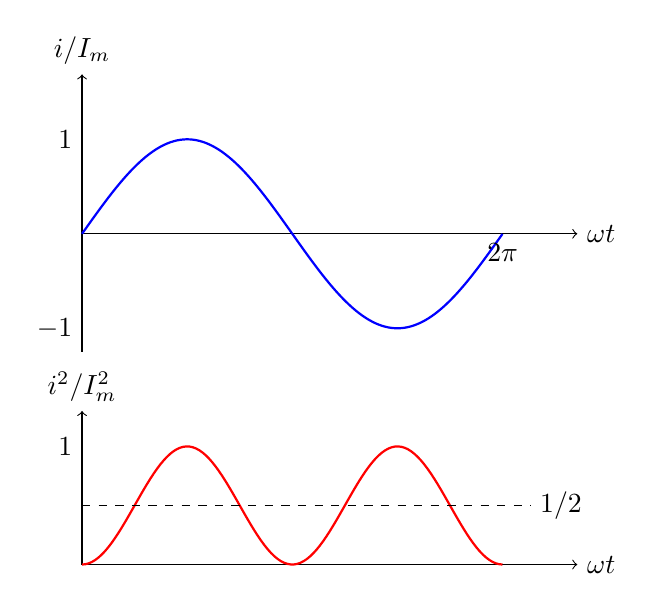
\begin{tikzpicture}[x=.85cm,y=.75cm]
\draw[->](0,0)--(7.4,0)node[right]{$\omega t$};\draw[->](0,-2)--(0,2.7)node[above]{$i/I_m$};
\draw[blue,thick,domain=0:6.283,samples=130]plot(\x,{1.6*sin(\x r)});\node[below]at(6.283,0){$2\pi$};\node[left]at(0,1.6){$1$};\node[left]at(0,-1.6){$-1$};
\begin{scope}[yshift=-4.2cm]\draw[->](0,0)--(7.4,0)node[right]{$\omega t$};\draw[->](0,0)--(0,2.6)node[above]{$i^2/I_m^2$};
\draw[red,thick,domain=0:6.283,samples=130]plot(\x,{2*sin(\x r)^2});\draw[dashed](0,1)--(6.7,1)node[right]{$1/2$};\node[left]at(0,2){$1$};\end{scope}
\end{tikzpicture}}
图\ref{fv:f6:rms}上图一个周期的有向面积为零，说明电流代数平均为零；下图平方始终非负，平均值为 $I_m^2/2$。电阻发热由 $R\int i^2\dd t$决定，与产生同样热量的直流相比，故 $I_{\rm rms}=I_m/\sqrt2$。这个系数只属于正弦波；半波整流、削顶或脉冲电流都应对其实际波形重新平方积分，不能只从峰值直接换算。




交流电中的有效值只把平方平均转换成等效直流数值，并不自动保留相位。电阻的平均功率可直接写成 $U^2/R$，但含电感、电容的负载需要有功分量。瞬时电源功率有时为负，表示储能元件把能量送回电源；一周期平均后，理想电抗元件的净功为零。发电机电磁转矩也随瞬时 $ei$ 改变，不能仅凭某一时刻电流正向就判断转矩恒为制动。


\section{从微分关系推导感抗、容抗与相量}

以正弦电流 $i=\sqrt2I\cos\omega t$ 为参考，理想电感端电压由微分给出：\[u_L=L\dot i=\sqrt2LI(-\sin\omega t)\omega=-\sqrt2\omega LI\sin\omega t=\sqrt2\omega LI\cos(\omega t+\pi/2).\]因此电感电压超前电流四分之一周期，感抗 $X_L=\omega L$。电容满足 $i=C\dot u_C$，因 $\dd(\sin\omega t)/\dd t=\omega\cos\omega t$，积分为
\[
 u_C(t)=\frac{\sqrt2I}{C}\int\cos\omega t\dd t
 =\frac{\sqrt2I}{\omega C}\sin\omega t+K.
\]
正弦项周期平均为零，无直流偏置要求 $K=0$，得到 $u_C=\sqrt2I\sin\omega t/(\omega C)$，即电压滞后电流四分之一周期，容抗 $X_C=1/(\omega C)$。

\fig{em6:series-rlc-real}{串联RLC的实际连接及被动电压正向；相量图必须对应同一参考电流}{\begin{tikzpicture}

\draw[world](0,0)--(1.5,0) (1.9,0)--(4,0) (0,2.4)--(1.2,2.4) (2,2.4)--(4,2.4) (0,0)--(0,.85) (0,1.55)--(0,2.4) (4,0)--(4,.35) (4,1.95)--(4,2.4);
\draw[world](0,1.2)circle(.35);\node at(0,1.2){$\sim$};\node[left]at(-.4,1.2){$u$};\node[left]at(0,1.8){$+$};\draw[world](1.2,2.2)rectangle(2,2.6);\node[above]at(1.6,2.65){$R$};\node[above]at(1.1,2.8){$+$};\node[above]at(2.1,2.8){$-$};
\foreach\j in {0,...,3}{\draw[world](4,{.35+.4*\j})arc(-90:90:.2);}\node[right]at(4.4,1.1){$L$};\node[right]at(4.2,2){$+$};\node[right]at(4.2,.2){$-$};
\draw[world](1.5,-.4)--(1.5,.4) (1.9,-.4)--(1.9,.4);\node at(1.7,-.95){$-\quad C\quad+$};\draw[flow,red](2.5,2.4)--(3.5,2.4)node[midway,above]{$i$};

\end{tikzpicture}}
图\ref{em6:series-rlc-real}沿电流方向经过每个元件，均以电流流入端为正端，故瞬时关系为 $u=u_R+u_L+u_C$。电流正向经过下侧电容时从右向左，电容的正端也必须画在右侧；若只沿元件在纸上的左右位置猜测端压正负，相量合成便会与实际回路不符。


相量是记录幅度与相位的复数工具，不是实际空间中的力矢量。采用有效值相量和 $\mathrm j^2=-1$，微分对应乘 $\mathrm j\omega$，故电感阻抗为 $\mathrm j\omega L$，电容阻抗为 $1/(\mathrm j\omega C)$。同频正弦稳态中可以使用相量的基尔霍夫方程；初始暂态、不同频率以及二极管开关过程不能直接用一个相量描述全过程。

串联 RLC 电路的电流相同，电阻电压与电流同相，电感、电容电压方向相反，所以
\[Z=R+\mathrm j(X_L-X_C),\quad |Z|=\sqrt{R^2+(X_L-X_C)^2},\quad I=U/|Z|.\]
相位满足 $\tan\phi=(X_L-X_C)/R$，功率因数 $\cos\phi=R/|Z|$。必须先合成正交相量，再取大小，不能把 $U_R,U_L,U_C$ 的有效值按普通正数相加。若已知三个电压大小而不知道接法，单凭大小关系也不能判断总电压。

\fig{em6:phasor}{串联电路电压的相量合成}{\begin{tikzpicture}[scale=.88]\draw[flow](0,0)--(3,0)node[right]{$U_R$};\draw[flow](3,0)--(3,2.8)node[above]{$U_L$};\draw[flow](3.6,2.8)--(3.6,1.4)node[midway,right]{$U_C$};\draw[guide](3,2.8)--(3.6,2.8) (3,1.4)--(3.6,1.4);\draw[force](0,0)--(3,1.4)node[midway,above]{$U$};\node[below]at(1.5,0){$I$ 为相位参考};\end{tikzpicture}}
图\ref{em6:phasor}先沿水平放置与电流同相的电阻电压，再把超前的电感电压向上相加、滞后的电容电压向下相加。总相量的竖直分量因而为$U_L-U_C$，斜边长度由勾股关系求出；图中上、下方向记录相位差，并非元件在空间中的摆放方向。

\subsection{复功率与补偿电流的物理意义}

使用有效值相量，复功率定义为 $S_c=\underline U\,\underline I^*=P+\mathrm jQ$，星号表示共轭。若阻抗为 $R+\mathrm jX$，则 $P=I^2R$、$Q=I^2X$，感性负载无功取正、容性负载取负。视在功率的大小为 $UI=\sqrt{P^2+Q^2}$，它反映线路与设备所承担的电压电流容量，不等同于每秒净消耗的能量。

\fig{em6:reactive-power-time}{理想电感中的电压、电流及瞬时功率；负功率时磁场返还能量}{\begin{tikzpicture}

\draw[axis](-.2,0)--(6.9,0)node[right]{$\omega t$};\draw[axis](0,-1.5)--(0,1.6)node[above]{$u/U_m,\ i/I_m$};
\draw[blue,thick,domain=0:6.283,samples=120]plot(\x,{cos(\x r)});\draw[red,thick,domain=0:6.283,samples=120]plot(\x,{-sin(\x r)});\node[blue]at(2.5,1.7){$i/I_m$};\node[red]at(4.5,1.7){$u/U_m$};
\begin{scope}[yshift=-4cm]\draw[axis](-.2,0)--(6.9,0)node[right]{$\omega t$};\draw[axis](0,-1.5)--(0,1.6)node[above]{$p/(UI)$};\draw[world,domain=0:6.283,samples=160]plot(\x,{-sin(2*\x r)});\node at(3.3,-2){一周期 $\int p\dd t=0$，瞬时 $p$ 可正可负};\end{scope}

\end{tikzpicture}}
图\ref{em6:reactive-power-time}取 $i=I_m\cos\omega t$，电感端压为 $u=-\omega LI_m\sin\omega t$，因此 $p=-UI\sin2\omega t$。这也等于磁场能的时间导数，链式法则给出
\[
 \frac{\dd}{\dd t}\left(\frac{LI_m^2}{2}\cos^2\omega t\right)
 =\frac{LI_m^2}{2}\,2\cos\omega t(-\sin\omega t)\omega
 =-\frac{\omega LI_m^2}{2}\sin2\omega t=-UI\sin2\omega t.
\]平均功率为零只说明一周期净储能变化为零，不能将任意瞬间的电压、电流或能量交换都置零。


给感性负载并联电容时，电容提供超前电流，减小电源端所需无功电流。在电源电压不变、原负载状态不变的条件下，负载本身有功功率不变，而线路电流可下降。若负载原来 $P,Q$ 已知，希望补偿到单位功率因数，所需电容满足 $\omega CU^2=Q$。过度补偿会使总负载呈容性，并不意味着线路电流可无限减小。

\fig{em6:compensation-circuit}{并联补偿保持负载端有效电压 $U$ 不变，电源电流等于两支路电流相量之和}{\begin{tikzpicture}

\draw[world](0,0)--(6,0)--(6,.9) (6,1.3)--(6,2.4)--(0,2.4)--(0,1.55) (0,.85)--(0,0) (3,0)--(3,.7) (3,1.7)--(3,2.4);
\draw[world](0,1.2)circle(.35);\node at(0,1.2){$\sim$};\node[left]at(-.4,1.2){$U$};\draw[world](2.7,.7)rectangle(3.3,1.7);\node at(3,1.2){$Z_L$};\draw[world](5.55,.9)--(6.45,.9) (5.55,1.3)--(6.45,1.3);\node[right]at(6.55,1.1){$C$};
\draw[flow,red](.7,2.4)--(1.8,2.4)node[midway,above]{$\underline I$};\draw[flow,blue](3.7,2.2)--(3.7,1.5)node[right]{$\underline I_L$};\draw[flow,blue](6.9,2.2)--(6.9,1.5)node[right]{$\underline I_C$};

\end{tikzpicture}}
图\ref{em6:compensation-circuit}中的电容与负载跨接同一对节点，故电容无功为 $Q_C=-\omega CU^2$。补偿不改变 $Z_L$ 及其端压时，负载支路的 $P,Q$ 保持原值，改变的是电源端相量和；若端压也随线路压降明显变化，就应同时求新的负载工作状态。


\fig{em6:compensation-current}{电压为水平相位参考时，并联电容改变电源所需无功电流}{
\begin{tikzpicture}[scale=1.1]
\draw[axis](-.2,0)--(4.3,0)node[right]{与$\underline U$同相};
\draw[axis](0,-2.5)--(0,1.1)node[above]{超前$90^\circ$};
\draw[force,blue](0,0)--(3,-2)node[midway,below left]{$\underline I_L$};
\draw[flow,red](3,-2)--(3,-.5)node[midway,right]{$\underline I_C$};
\draw[force](0,0)--(3,-.5)node[midway,above]{$\underline I$};
\draw[guide](3,-2)--(3,0);
\node[above]at(3,0){$I_P=P/U$};
\node[below]at(1.9,-2.8){$\underline I=\underline I_L+\underline I_C$};
\end{tikzpicture}}

图\ref{em6:compensation-current}中感性负载电流$\underline I_L$滞后电压，竖直分量向下；电容电流$\underline I_C$向上。两者相加后，水平分量$I_P=P/U$不变，向下的无功分量由$Q/U$减为$(Q-\omega CU^2)/U$，故
\[
 I=\frac{\sqrt{P^2+(Q-\omega CU^2)^2}}{U}.
\]
图中红箭头恰好抵消全部竖直分量时，电源电流最小，为$P/U$；继续加大电容会使合电流超前并重新增大。线路损耗据这一合电流计算，负载支路电流本身并未因理想并联补偿而减小。


测量总功率时，理想电感电容的平均功率为零不等于可以从电流合成中删去它们。线路电阻对全部线路电流发热，无功电流同样增加 $I^2R$ 损耗。提高功率因数能降低线路损耗，是改变相量分配的结果，不能通过把某个仪表读数直接换成有功电流来计算。


\section{串并联谐振与实际线圈}

串联谐振满足 $X_L=X_C$，角频率 $\omega_0=1/\sqrt{LC}$，输入阻抗等于 $R$、电流最大。此时电感和电容各自电压可以远高于电源电压，因为两者相量抵消；电容端高电压并不违反回路电压定律。电压放大倍数在谐振时为 $\omega_0L/R$，实际损耗和元件耐压限制其大小。

并联电路各支路电压相同，应先加电流相量。理想 $L,C$ 并联的无功电流分别滞后、超前电压 $90^\circ$，在 $\omega C=1/(\omega L)$ 时抵消。输入电流可以很小，而支路电流仍很大。若有并联电阻，电源仍供给它所需的有功电流；不能把谐振理解为所有支路都无电流。

\fig{em6:parallel-resonance-real}{并联RLC的共同端压与支路电流参考；谐振抵消的是电感、电容电流相量}{\begin{tikzpicture}

\draw[world](0,0)--(6,0) (0,2.4)--(6,2.4) (0,0)--(0,.7) (0,1.7)--(0,2.4);\draw[world](-.2,.7)rectangle(.2,1.7);\node[left]at(-.3,1.2){$R$};
\draw[world](3,0)--(3,.35) (3,1.95)--(3,2.4);\foreach\j in {0,...,3}{\draw[world](3,{.35+.4*\j})arc(-90:90:.2);}\node[left]at(2.8,1.2){$L$};\draw[world](6,0)--(6,.9) (6,1.3)--(6,2.4);\draw[world](5.55,.9)--(6.45,.9) (5.55,1.3)--(6.45,1.3);\node[right]at(6.55,1.1){$C$};
\draw[flow,red](1.3,3.2)--(1.3,2.5)node[midway,right]{$\underline I$};\draw[flow](3.7,2.1)--(3.7,1.5)node[right]{$\underline I_L$};\draw[flow](6.9,2.1)--(6.9,1.5)node[right]{$\underline I_C$};\node at(3,-.7){共同端压 $\underline U$，$\underline I=\underline U/R+\underline I_L+\underline I_C$};

\end{tikzpicture}}
在图\ref{em6:parallel-resonance-real}中，输入导纳为 $Y=1/R+\mathrm j[\omega C-1/(\omega L)]$。谐振时虚部为零，电源仍供给 $U/R$ 的同相电流，而两个电抗支路的电流大小相等、相位相反。串联谐振通过电压抵消使输入阻抗最小，并联谐振则通过电流抵消使输入导纳的模最小，两者应按各自实际连接讨论。


实际线圈通常包含串联电阻 $r$，其阻抗为 $r+\mathrm j\omega L$，电压相位不再恰好超前 $90^\circ$。线圈与纯电阻并联时，可以用总有功功率确定线圈电流的同相分量，再结合总电流求其无功分量。还应检查线圈的有功功率非负、等效电阻非负，避免选取没有物理意义的代数根。


\subsection{谐振曲线、半功率带宽与测量条件}

固定有效电压驱动的串联 RLC，电流为 $I(\omega)=U/\sqrt{R^2+(\omega L-1/(\omega C))^2}$。远低于谐振频率时容抗主导，电流随频率上升而增大；远高于谐振频率时感抗主导，电流反而减小。最大电流出现在两者抵消处，峰值为 $U/R$。因此谐振提高的是特定频段的响应，不是对任意频率都有相同放大。

当电流下降到峰值的$1/\sqrt2$，电阻功率恰为最大值的一半。
\fig{em6:resonance-band}{串联RLC的归一化谐振曲线；半功率点对应电流峰值的$1/\sqrt2$}{
\begin{tikzpicture}[x=2.7cm,y=2.7cm]
\draw[axis](0,0)--(2.65,0)node[right]{$\omega/\omega_0$};
\draw[axis](0,0)--(0,1.25)node[above]{$I/(U/R)$};
\draw[world,blue,domain=.03:2.5,samples=220]
 plot(\x,{1/sqrt(1+9*(\x-1/\x)^2)});
\draw[guide](0,.707107)--(1.9,.707107);
\draw[guide](.847127,0)--(.847127,.707107)
 (1,0)--(1,1) (1.18046,0)--(1.18046,.707107);
\fill(.847127,.707107)circle(.6pt);
\fill(1.18046,.707107)circle(.6pt);
\node[left]at(0,1){$1$};
\node[left]at(0,.707107){$1/\sqrt2$};
\node[below]at(.78,0){$\omega_-/\omega_0$};
\node[above right]at(1,1){谐振峰};
\node[below]at(1.3,0){$\omega_+/\omega_0$};
\draw[dim](.847127,-.43)--(1.18046,-.43);
\node[below]at(1,-.43){$\Delta\omega/\omega_0$};
\end{tikzpicture}}

图\ref{em6:resonance-band}图示$Q_f=3$。曲线的高度只在$\omega=\omega_0$处为一，而两侧交点满足
\[
 \frac{U^2}{R^2+(\omega L-1/\omega C)^2}
     =\frac{U^2}{2R^2},
 \qquad \omega L-\frac1{\omega C}=\pm R.
\]
两边乘以正量 $\omega$，高频侧满足 $L\omega^2-R\omega-1/C=0$，低频侧满足 $L\omega^2+R\omega-1/C=0$。用求根公式，各方程舍去负根，得到
\[
 \omega_\pm=\frac{\sqrt{R^2+4L/C}\pm R}{2L},\qquad
 \Delta\omega=\omega_+-\omega_-=\frac RL,\quad
 \omega_+\omega_-=\frac1{LC}.
\]
图中横坐标是角频率；改用频率$f$时带宽应除以$2\pi$。两半功率点关于$\omega_0$并不严格算术对称，其几何平均才等于$\omega_0$。

定义品质因数$Q_f=\omega_0L/R$，在上述固定$R,L,C$的串联模型中，$\Delta\omega/\omega_0=1/Q_f$。弱阻尼还使振荡频率接近$\omega_0$，但并非带宽等式成立的必要条件。这里的品质因数符号与电荷、无功功率不同，写式时应保留区分。

真实线圈电阻随频率改变、元件存在寄生电容时，上述理想曲线会发生变化。交流表的有效值读数还依赖仪表是否按真有效值测量；只针对正弦波校准的平均值响应表，在截波与脉冲电流中可能不能直接显示定义上的均方根值。理想题目给出的“有效值表”应理解为符合相应测量定义，而非所有现实电表在所有频率都完全一样。

限幅后的电表读数可承接图\ref{em6:clipper-waveforms}计算。相位边界已由阈值确定，选择仪表模型以后，还应明确它测的是全波形有效值、交流分量有效值，还是按正弦校准的平均响应值；三种定义对同一截波可能给出不同读数。



\subsection{由半功率点识别参数}

串联谐振的参数识别可承接图\ref{em6:resonance-band}。已知串联电阻$R$并测出两半功率角频率，由它们的差和积依次求
\[
 L=\frac{R}{\omega_+-\omega_-},\qquad
 C=\frac{1}{L\omega_+\omega_-}.
\]
还应检查实测峰值是否为$U/R$、峰频是否为$\sqrt{\omega_+\omega_-}$。只有这些结果相容，才能把观测解释为该串联模型。用角频率还是频率必须贯穿一致，不能漏掉$2\pi$。


\section{二极管分段与非正弦波形}

理想二极管导通时端压为零且电流只能沿允许方向；截止时电流为零且两端反向偏置。含直流偏置的限幅电路，应先假设截止，求开路二极管两端电压，再判定何时正向；在导通区间用短路替代二极管，重新求输出，并检查电流方向。边界处通常由两段输出相等确定。

并联限幅通过导通支路钳住输出电压，串联限幅则通过切断传输路径使输出成为零或某个固定偏置，二者不能仅凭“峰值超过阈值”使用同一波形。画图前需标清输入输出参考端、直流源极性、二极管方向及负载位置。求有效值和平均值时，根据各导通区间分别积分，不能再把输入的正弦有效值当成输出。

\fig{em6:clipper-circuits}{正向阈值相同的两种接法；二极管三角端到横杠为允许电流方向}{
\begin{tikzpicture}[scale=.83]
\begin{scope}
\node at(1.6,4){并联上限钳位（高阻输出）};
\draw[world](0,0)--(3.2,0)
 (0,0)--(0,1) (0,1.8)--(0,2.7)--(1,2.7)
 (2,2.7)--(3.2,2.7)--(4.1,2.7);
\draw[world](0,1.4)circle(.4)node{$u_i$};
\node[left]at(-.4,2){$+$};
\draw[world](1,2.52)rectangle(2,2.88);
\node[above]at(1.5,2.9){$R$};
\draw[world](3.2,2.7)--(3.2,2.15);
\draw[world](2.95,2.15)--(3.45,2.15)--(3.2,1.7)--cycle;
\draw[world](2.9,1.65)--(3.5,1.65);
\draw[world](3.2,1.65)--(3.2,1.15) (3.2,.35)--(3.2,0);
\draw[world](3.2,.75)circle(.4)node{$E_b$};
\node[left]at(2.7,1.1){$+$};
\node[right]at(3.55,1.95){$D$};
\fill(3.2,2.7)circle(1.5pt);
\node[right]at(4.1,2.7){$u_o$};
\node[below]at(1.6,0){共同参考端};
\end{scope}
\begin{scope}[xshift=7cm]
\node at(1.8,4){串联阈值传输};
\draw[world](0,0)--(4,0)--(4,.7) (4,1.7)--(4,2.7)--(3,2.7)
 (2.2,2.7)--(1.7,2.7) (1.2,2.7)--(0,2.7)--(0,1.8) (0,1)--(0,0);
\draw[world](0,1.4)circle(.4)node{$u_i$};
\node[left]at(-.4,2){$+$};
\draw[world](1.2,2.45)--(1.2,2.95)--(1.65,2.7)--cycle;
\draw[world](1.7,2.4)--(1.7,3);
\node[above]at(1.4,3){$D$};
\draw[world](2.6,2.7)circle(.4)node{$E_b$};
\node[above]at(2.15,2.95){$+$};
\draw[world](3.82,.7)rectangle(4.18,1.7);
\node[right]at(4.3,1.2){$R_L$};
\node[right]at(4,2.7){$u_o$};
\node[below]at(1.8,0){共同参考端};
\end{scope}
\end{tikzpicture}}

图\ref{em6:clipper-circuits}取$u_i=U_m\sin\varphi$、$0<E_b<U_m$，输出均对下方公共导线计。左图截止时电阻无电流，$u_o=u_i$；一旦$u_i>E_b$，二极管把输出钳在$E_b$，并有正向电流$(u_i-E_b)/R$。右图截止时负载电流为零，故$u_o=0$；导通时沿串联路径扣除$E_b$，得到$u_o=u_i-E_b$。于是
\[
 u_{o,\text{并}}=\min(u_i,E_b),\qquad
 u_{o,\text{串}}=\max(u_i-E_b,0).
\]
左图采用高阻测量端，若输出并接有限负载，截止时还需先计算电阻分压，阈值也随之改变。

\fig{em6:clipper-waveforms}{同一正弦输入的两种输出；图示$E_b/U_m=1/2$，虚线为输入}{
\begin{tikzpicture}[x=.8cm,y=1.25cm]
\foreach \shift/\mode in {0/0,8/1}{
\begin{scope}[xshift=\shift cm]
\draw[axis](0,0)--(6.8,0)node[right]{$\varphi$};
\draw[axis](0,-1.15)--(0,1.4)node[above]{$u/U_m$};
\draw[guide,gray,domain=0:6.283,samples=100]plot(\x,{sin(\x r)});
\draw[guide](0,.5)--(3.3,.5);
\draw[guide](.5236,-1.05)--(.5236,1.05) (2.618,-1.05)--(2.618,1.05);
\node[below]at(.5236,-1.05){$\alpha$};
\node[below]at(2.618,-1.05){$\pi-\alpha$};
\node[left]at(0,.5){$E_b/U_m$};
\ifnum\mode=0
\draw[world,blue,domain=0:6.283,samples=180]plot(\x,{min(sin(\x r),.5)});
\node at(3.1,-1.8){并联：削去正峰顶部};
\else
\draw[world,blue,domain=0:6.283,samples=180]plot(\x,{max(sin(\x r)-.5,0)});
\node at(3.1,-1.8){串联：只传输超过阈值的部分};
\fi
\end{scope}}
\end{tikzpicture}}

图\ref{em6:clipper-waveforms}的两条竖虚线由$U_m\sin\alpha=E_b$确定。在区间$[\alpha,\pi-\alpha]$内二极管导通，但左图输出是常量、右图输出仍随输入变化；同一导通区间并不意味着同一输出。求平均值、有效值时，先按图写出各段函数，再对完整周期$0\le\varphi<2\pi$积分。


具有发光阈值的器件还涉及导通占空时间。简化模型若假定正负极性均在 $|u|\ge U_b$ 时发光，则用两半周的对称区间计算；若仅允许一个方向发光，时间应减少为相应单半周。真实辉光管有维持电压、熄灭电压和限流要求，题目中的单一阈值只是理想化计时模型。



非正弦波形应从定义重新积分。整流、截波和限幅通常保持周期性，却改变导通区间，正弦峰值除以 $\sqrt2$ 的结论不再适用。积分时必须用整个周期归一化，不能只在导通区间求平均。对于带直流分量的输出，平均电压描述电荷净输运，有效电压描述热效应，纹波有效值则需先减去直流分量再平方平均，三者不能互换。

\subsection{电容滤波与小纹波近似}

电容滤波把短时间补充电荷与较长时间向负载放电联系起来。小纹波近似下，先以相邻充电峰的间隔估计电荷缺额，再求峰谷差及平均输出。理想零电阻充电可能给出不可接受的尖峰电流，平均输出近似不能用于确定二极管峰值额定电流；这需要增加电源内阻和有限导通时间。


\fig{em6:rectifier-filter}{半波整流后的电容滤波：峰值附近补充电荷，其余时间由电容向负载放电}{\begin{tikzpicture}

\draw[world](0,0)--(6,0)--(6,.7) (6,1.7)--(6,2.4)--(2.5,2.4) (2,2.4)--(1.6,2.4) (.9,2.4)--(0,2.4)--(0,1.55) (0,.85)--(0,0);\draw[world](0,1.2)circle(.35);\node at(0,1.2){$\sim$};\node[left]at(-.4,1.2){$u_i$};
\draw[world](.9,2.2)rectangle(1.6,2.6);\node[above]at(1.25,2.65){$r_s$};\draw[world](2,2.15)--(2,2.65)--(2.45,2.4)--cycle;\draw[world](2.5,2.1)--(2.5,2.7);\node[above]at(2.25,2.85){$D$};
\draw[world](4,0)--(4,.9) (4,1.3)--(4,2.4);\draw[world](3.55,.9)--(4.45,.9) (3.55,1.3)--(4.45,1.3);\node[left]at(3.5,1.1){$C$};\draw[world](5.8,.7)rectangle(6.2,1.7);\node[right]at(6.3,1.2){$R_L$};\node[right]at(6,2.4){$u_o$};

\end{tikzpicture}}
在图\ref{em6:rectifier-filter}中，二极管只在输入足以补充电容电荷时导通。对电阻负载，在截止段由 $C\dot u=-u/R_L$ 得
\[
 \int_{U_{\max}}^{u(t)}\frac{\dd z}{z}
 =-\frac1{R_LC}\int_0^t\dd s,\qquad
 u(t)=U_{\max}\e^{-t/(R_LC)}.
\]
若 $t/(R_LC)\ll1$，展开指数为 $u(t)\simeq U_{\max}[1-t/(R_LC)]$，即近似线性放电。若峰间放电电流近似为 $I_L$、相邻充电峰间隔为 $1/f_r$，电荷缺额由
$\Delta q=\int_0^{1/f_r}I_L\dd t=I_L[t]_0^{1/f_r}=I_L/f_r$ 给出，从而
\[\Delta U\simeq\frac{I_L}{f_rC},\qquad
\overline U_o\simeq U_{\max}-\frac{\Delta U}{2}.\]
半波整流 $f_r=f$，全波整流 $f_r=2f$。电阻负载下还需 $I_L\simeq\overline U_o/R_L$，并检查 $f_rR_LC\gg1$ 才能把放电段近似为小斜率。忽略二极管压降及电源内阻引起的峰值下降时，$U_{\max}$ 才近似等于输入峰值。小纹波近似描述输出电压，不能据此推断充电尖峰电流；后者仍受 $r_s$ 与有限导通区间控制。

对任何周期输出，令直流分量 $U_{\rm dc}=\overline u_o$、交流分量 $u_{\rm ac}=u_o-U_{\rm dc}$。展开平方并利用 $\overline{u_{\rm ac}}=0$，有
\[U_{\rm rms}^2=U_{\rm dc}^2+U_{\rm ac,rms}^2.\]
因此平均值、完整有效值和纹波有效值对应不同的测量定义，不能只凭一个峰谷差互相替代。


\section{变压器的端口与负载折算}

理想变压器的两绕组链接相同主磁通，$e_1=-N_1\dot\Phi,e_2=-N_2\dot\Phi$。忽略线阻、漏磁和铁芯损耗，端电压有效值之比为 $U_1/U_2=N_1/N_2$。在理想无励磁电流极限，负载电流所产生的磁动势互相抵消，电流大小满足 $N_1I_1=N_2I_2$，相位与绕组同名端相容；输入输出有功功率相等。不能只用功率相等推断所有有相位差负载的瞬时电流方向。

匝数比 $n=N_1/N_2$，副边阻抗 $Z_2$ 折算到原边为 $Z_1=n^2Z_2$，这可以从电压和电流比直接相除得到。普通变压器需要变化的磁通；恒定直流接入真实原边可能形成很大电流，不能用交流稳态匝比公式推断正常直流变压。

\fig{em6:transform}{电压均按同名端对非同名端取值；原边电流流入圆点端，副边负载电流从圆点端流出}{\begin{tikzpicture}
\draw[world](0,2.4)--(0,1.95);\draw[world](0,0.35)arc(-90:90:.2);\draw[world](0,0.75)arc(-90:90:.2);\draw[world](0,1.15)arc(-90:90:.2);\draw[world](0,1.5500000000000003)arc(-90:90:.2);\draw[world](0,.35)--(0,0);\fill(-0.22,2.15)circle(2pt);\draw[world](3.5,2.4)--(3.5,1.95);\draw[world](3.5,0.35)arc(-90:90:.2);\draw[world](3.5,0.75)arc(-90:90:.2);\draw[world](3.5,1.15)arc(-90:90:.2);\draw[world](3.5,1.5500000000000003)arc(-90:90:.2);\draw[world](3.5,.35)--(3.5,0);\fill(3.28,2.15)circle(2pt);
\draw[world](1.5,-.2)--(1.5,2.6) (1.7,-.2)--(1.7,2.6);\node[left]at(-.4,1.1){$N_1$};\node[left]at(3.1,1.1){$N_2$};
\draw[world](3.5,2.4)--(6,2.4)--(6,1.7) (6,.7)--(6,0)--(3.5,0);\draw[world](5.8,.7)rectangle(6.2,1.7);\node[right]at(6.3,1.2){$Z_2$};
\draw[flow,red](0,3.2)--(0,2.5)node[midway,right]{$\underline I_1$};\draw[flow,red](4,2.4)--(5,2.4)node[midway,above]{$\underline I_2$};
\node[left]at(-.1,2.4){$+$};\node[left]at(-.1,0){$-$};\node[right]at(3.6,2.35){$+$};\node[right]at(3.6,0){$-$};\node at(0,-.65){$\underline U_1$};\node at(3.5,-.65){$\underline U_2$};

\end{tikzpicture}}
图\ref{em6:transform}的两绕组共用铁芯主磁通，因此两边每匝的感应电动势相同。沿图中的副边负载回路求电流后，再由安匝关系折算到原边；负载断开时理想模型的两边负载电流均为零。图中的两条铁芯线只示意主磁路，匝比关系还依赖前述忽略漏磁与损耗的条件。


理想变压器的副边负载若为电阻 $R_L$，原边看到 $n^2R_L$，因此原边电流既由匝数比决定，也受负载控制。副边开路时理想负载电流为零；副边负载电阻减小，原边电流随之增大。不能把变压器误看成只规定电压、而原边电流永远固定的装置。真实变压器还需要励磁电流，本讲的理想模型把它忽略。


图\ref{em6:transform}采用副边向负载送出的电流正向，因此理想安匝平衡写为 $N_1\underline I_1=N_2\underline I_2$，电压比为 $\underline U_1=n\underline U_2$。两式相除即得 $Z_1=\underline U_1/\underline I_1=n^2Z_2$。若把副边参考改成流入圆点端，则电流关系须增加负号；电压比和功率关系也要保持同一套参考。


\subsection{负载匹配与效率极值}

变压器在改变电压的同时还改变源端看到的负载阻抗。给定实际负载时，选择匝比相当于选择折算阻抗；最大输出功率由负载与源内阻的匹配决定，而不是单纯追求最高次级电压。最高效率与最大功率通常属于不同的工作点。真实变压器的恒定铁损与随电流平方增大的铜损，也会使效率在某一负载处达到极值。

求极值应先写清哪些量固定。例如以理想稳压次级电压为常量求最佳电流时，可以把输出功率写成 $UI$；若负载变化导致明显电压调整率，就需要把 $U(I)$ 一并代入。数学极值只有在模型允许的电流、温升和额定电压范围内才有实际意义。


\fig{em6:load-matching}{通过理想变压器改变折算负载；有内阻的交流源最大输出功率出现在阻抗匹配点}{\begin{tikzpicture}

\draw[axis](-.2,0)--(6.5,0)node[right]{$z=n^2R_L/r_s$};\draw[axis](0,-.2)--(0,2.7)node[above]{$P_L/P_{\max},\ \eta$};
\draw[world,blue,domain=0:6,samples=100]plot(\x,{8*\x/(1+\x)^2});\draw[world,red,domain=0:6,samples=100]plot(\x,{2*\x/(1+\x)});
\draw[guide](1,0)--(1,2)--(0,2);\fill(1,2)circle(2pt);\node[below]at(1,0){$1$};\node[left]at(0,2){$1$};\node[blue]at(3.5,2.6){输出功率};\node[red]at(4.8,1.9){源到负载效率};

\end{tikzpicture}}
若电源有效电动势 $E$、串联内阻 $r_s>0$ 固定，理想变压器副边接电阻 $R_L$，令折算电阻 $R'=n^2R_L$，则
\[
P_L=\frac{E^2R'}{(r_s+R')^2}.
\]
固定 $E,r_s$，使用乘积法则与幂函数求导：
\begin{align*}
\frac{\dd P_L}{\dd R'}
&=E^2\left[(r_s+R')^{-2}-2R'(r_s+R')^{-3}\right]\\
&=\frac{E^2[(r_s+R')-2R']}{(r_s+R')^3}
=\frac{E^2(r_s-R')}{(r_s+R')^3}.
\end{align*}
图\ref{em6:load-matching}的功率峰值对应 $R'=r_s$、$n=\sqrt{r_s/R_L}$，$P_{\max}=E^2/(4r_s)$。此时源内阻损耗等于负载功率，源到负载效率为 $1/2$；增大折算负载可提高效率，却会使输出功率最终趋零。因此最大功率与最高效率不能按同一极值处理。

真实变压器若输出有效电压 $U$ 近似恒定，铁损 $P_0$ 近似恒定、铜损为 $\beta I^2$，则
\[
\eta(I)=\frac{UI}{UI+P_0+\beta I^2}.
\]
分子、分母对 $I$ 的导数分别为 $U$ 和 $U+2\beta I$，商法则给出
\begin{align*}
\eta'(I)
&=\frac{U(UI+P_0+\beta I^2)-UI(U+2\beta I)}
{(UI+P_0+\beta I^2)^2}\\
&=\frac{U(P_0-\beta I^2)}{(UI+P_0+\beta I^2)^2}.
\end{align*}
效率极大值出现在 $\beta I^2=P_0$，仍须落在该近似有效的额定工作范围内。这里改变的是实际损耗模型下的负载电流，与上一幅图通过匝比匹配源内阻的问题不同。


\section{三相连接与中性点约束}

平衡三相电源的三个相电压相差 $120^\circ$。星形连接时线电压是两个相电压之差，大小为 $\sqrt3U_\phi$，线电流等于相电流；三角形连接时线电压等于相电压，线电流是两支路电流之差，大小为 $\sqrt3I_\phi$。平衡有功功率均可写成 $\sqrt3U_\ell I_\ell\cos\phi$。星形中性线电流为三相电流相量和，平衡时为零，不平衡时不能继续删去中性线影响。

\fig{em6:connection-model}{星形与三角形的实际连接；各箭头仅规定电流正向}{\begin{tikzpicture}[scale=.85]
\begin{scope}
\node at(1.4,4.1){星形};
\coordinate(a)at(1.4,2.8);\coordinate(b)at(0,0);\coordinate(c)at(2.8,0);
\coordinate(n)at(1.4,1);
\draw[world](a)--(n)--(b) (n)--(c);
\node[draw,fill=white]at(1.4,1.95){$Z$};
\node[draw,fill=white]at(.7,.5){$Z$};
\node[draw,fill=white]at(2.1,.5){$Z$};
\draw[flow](1.4,3.75)--(a)node[midway,right]{$I_a$};
\draw[flow](-1,0)--(b)node[midway,above]{$I_b$};
\draw[flow](3.8,0)--(c)node[midway,above]{$I_c$};
\fill(n)circle(2pt)node[right]{$N$};
\draw[guide](n)--(1.4,-.65)node[below]{$O$};
\node[above left]at(a){$a$};\node[below left]at(b){$b$};\node[below right]at(c){$c$};
\end{scope}
\begin{scope}[xshift=7cm]
\node at(1.4,4.1){三角形};
\coordinate(a)at(1.4,2.8);\coordinate(b)at(0,0);\coordinate(c)at(2.8,0);
\draw[world](a)--(b)--(c)--cycle;
\node[draw,fill=white]at(.7,1.4){$Z$};
\node[draw,fill=white]at(2.1,1.4){$Z$};
\node[draw,fill=white]at(1.4,0){$Z$};
\draw[flow](1.4,3.75)--(a)node[midway,right]{$I_a$};
\draw[flow](-1,0)--(b)node[midway,above]{$I_b$};
\draw[flow](3.8,0)--(c)node[midway,above]{$I_c$};
\draw[flow,blue](1.15,2.3)--(.9,1.8)node[midway,left]{$I_{ab}$};
\draw[flow,blue](.4,0)--(.9,0)node[midway,below]{$I_{bc}$};
\draw[flow,blue](2.55,.5)--(2.3,1)node[midway,right]{$I_{ca}$};
\node[above left]at(a){$a$};\node[below left]at(b){$b$};\node[below right]at(c){$c$};
\end{scope}
\end{tikzpicture}
}
图\ref{em6:connection-model}左图每条线只接一个负载，所以$I_\ell=I_\phi$；右图节点$a$有两条负载支路，按图中箭头列节点方程为$\underline I_a=\underline I_{ab}-\underline I_{ca}$。星形中线电压是两端相电压之差，三角形中每个负载直接跨接在线端之间。连接关系先确定，再对相量差取模，才能得到$\sqrt3$因子。



三相功率公式也需要保持连接条件一致。星形改为三角形，在相同线电压、相同单相阻抗下，单相电压增大 $\sqrt3$ 倍，单相功率为原来的三倍，总功率同样增至三倍。若比较条件变成总功率固定，线电流与单相阻抗都要按新的条件求，不能继续沿用三倍关系。

\fig{em6:phase-voltage-difference}{星形线电压由相电压相减得到，不能将相电压大小直接相加}{\begin{tikzpicture}

\draw[axis](-1.7,0)--(3.7,0)node[right]{实部};\draw[axis](0,-2.3)--(0,2.4)node[above]{虚部};
\draw[flow,blue](0,0)--(2,0)node[below]{$\underline U_a$};\draw[flow,blue](0,0)--(-1,-1.732)node[below left]{$\underline U_b$};
\draw[flow,red](2,0)--(3,1.732)node[midway,right]{$-\underline U_b$};\draw[force](0,0)--(3,1.732)node[above]{$\underline U_{ab}$};\draw[world](.8,0)arc(0:30:.8);\node at(1.2,.32){$30^\circ$};
\node at(1,-2.9){$\underline U_{ab}=\underline U_a-\underline U_b$};

\end{tikzpicture}}
图\ref{em6:phase-voltage-difference}取 $\underline U_a=U_\phi$、$\underline U_b=U_\phi\e^{-\mathrm j2\pi/3}$。从 $\underline U_a$ 的箭头端再加 $-\underline U_b$，得到 $\underline U_{ab}=\sqrt3U_\phi\e^{\mathrm j\pi/6}$，所以线电压比相电压大 $\sqrt3$ 倍，并有相位差。三角形节点的电流相减以相同方法处理；只比较支路电流大小而不处理相位，会遗漏线电流的 $\sqrt3$ 因子。


\subsection{中性线断开后的浮动节点}

\fig{em6:neutral-topology}{不平衡星形负载的两种中性线状态；阻抗按支路标出}{
\begin{tikzpicture}[scale=.83]
\foreach \shift/\closed in {0/1,6.1/0}{
\begin{scope}[xshift=\shift cm]
\draw[world](0,2.4)--(2.1,1.2)--(0,0) (2.1,1.2)--(4.2,0);
\node[draw,fill=white]at(1.05,1.8){$Z_a$};
\node[draw,fill=white]at(1.05,.6){$Z_b$};
\node[draw,fill=white]at(3.15,.6){$Z_c$};
\node[left]at(0,2.4){$a$};\node[left]at(0,0){$b$};\node[right]at(4.2,0){$c$};
\fill(2.1,1.2)circle(2pt)node[above right]{$N$};
\draw[world](2.1,1.2)--(3,2.4) (3.6,2.4)--(4.2,2.4);
\node[right]at(4.2,2.4){$O$};
\ifnum\closed=1
\draw[world](3,2.4)--(3.6,2.4);
\node at(2.1,3.3){中性线完好：$V_N=V_O$};
\else
\draw[world](3,2.4)--(3.5,2.75);
\node at(2.1,3.3){中性线断开：$V_N$待求};
\fi
\end{scope}}
\end{tikzpicture}}

图\ref{em6:neutral-topology}左图由导线直接规定$V_N=V_O$。右图的开关断开后，应对浮动节点$N$列方程。相电压均对$O$计，令$\underline U_N=V_N-V_O$，得到
\[
 \sum_{j=a,b,c}\frac{\underline U_j-\underline U_N}{Z_j}=0,\qquad
 \underline U_N=
 \frac{\underline U_a/Z_a+\underline U_b/Z_b+\underline U_c/Z_c}
      {1/Z_a+1/Z_b+1/Z_c}.
\]
这里假定分母非零并存在有限的正弦稳态。各负载电压随后由$\underline U_{jN}=\underline U_j-\underline U_N$求出；三个阻抗相等时，相电压和为零使中性点位移恢复为零。若是特殊无损网络导致分母为零，应检查是否存在稳态，不能直接相除。


图\ref{em6:neutral-topology}中的断线改变了节点约束，电源的三个相电压仍保持原值，负载相电压却需重新求出。平衡时的中性线零电流只是三相电流相量和为零的特例，不能推广到任意不平衡负载。


\section{输电线路的电压与功率平衡}

输电线路耗散为 $I^2R_\ell$，用户得到的功率等于送出功率减线路损耗。变压器升压的作用，是在相同输送功率和功率因数下减小线路电流；不能只升电压而仍保持原来的线路电流计算损耗。受端电压应由送端电压扣除线路压降后再求降压匝比，两端变压器的匝比一般不同。



纯电阻输电线路中，送端 $U_s$、受端 $U_r$、线路电流 $I$ 满足 $U_s-U_r=IR_\ell$；功率差为 $(U_s-U_r)I=I^2R_\ell$。若损耗比例给的是占送出功率 $\eta$，则 $P_r=(1-\eta)P_s$；若给的是占用户功率，分母不同，应先换算再求电流。把这两种“损耗百分比”混同会同时影响两端变压器匝比。

对于有明显无功的交流长线路，电压降一般是相量关系，不能直接按正数 $U_s-U_r=IR$ 相减。本讲水电题采用功率因数为一、线路仅有电阻的模型，正数相减才成立。若扩展到感性负载，应把线路阻抗、负载相位和变压器折算一起纳入，而不是只在原公式后乘一个功率因数。


\fig{em6:transmission-balance}{功率因数为一时的线路模型；往返总电阻等效画在上支路}{\begin{tikzpicture}

\draw[world](0,0)--(6,0)--(6,.7) (6,1.7)--(6,2.4)--(3.5,2.4) (2.5,2.4)--(0,2.4)--(0,1.55) (0,.85)--(0,0);\draw[world](0,1.2)circle(.35);\node at(0,1.2){$\sim$};\node[left]at(-.4,1.2){$U_s$};\draw[world](2.5,2.2)rectangle(3.5,2.6);\node[above]at(3,2.65){$R_\ell$};\draw[world](5.8,.7)rectangle(6.2,1.7);\node[right]at(6.3,1.2){用户};\draw[flow,red](.7,2.4)--(1.8,2.4)node[midway,above]{$I$};\draw[flow,red](4.8,0)--(3.7,0);
\draw[dim](5,0)--(5,2.4)node[midway,left]{$U_r$};\node at(3,-.7){$U_sI=U_rI+I^2R_\ell$};

\end{tikzpicture}}
图\ref{em6:transmission-balance}把有功功率与线路电流放在同一个回路中检验。已知送端功率和允许损耗时，先由 $I^2R_\ell$ 求电流，再求送、受端电压；降压变压器应使用实际受端 $U_r$，不能仍用送端 $U_s$。若负载有无功分量，应先建立相量电压关系，图中的正数相减便不再适用。


\section{振荡电路与电磁波的联系}

电容板间没有传导电流穿过绝缘层，但变化电场仍对应磁场的环流。麦克斯韦引入位移电流 $I_d=\varepsilon_0\dd\Phi_E/\dd t$，使跨过导线截面或跨过极板间隙选取曲面时，安培环路关系给出一致的磁场。位移电流不是电子真的穿过真空间隙，而是电场变化对磁场的贡献。

\fig{em6:ampere-surfaces}{同一安培环路的两种张面；蓝色面截导线，红色面从极板外绕入间隙（示意剖面）}{
\begin{tikzpicture}[scale=.95]
\fill[blue!12](-2,0)ellipse(.35 and 1.05);
\draw[red,dashed](-2,1.05)..controls(-1.3,2.2)and(.4,2.2)..(.4,1.1)
 ..controls(.7,.6)and(.7,-.6)..(.4,-1.1)
 ..controls(.4,-2.2)and(-1.3,-2.2)..(-2,-1.05);
\draw[world,very thick](-.6,-1.4)--(-.6,1.4) (.9,-1.4)--(.9,1.4);
\draw[world](-3.4,0)--(-.6,0) (.9,0)--(2.6,0);
\draw[world,blue](-2,0)ellipse(.35 and 1.05);
\draw[flow](-3.1,0)--(-2.5,0)node[midway,above]{$I$};
\foreach \y in {-.7,0,.7}
 \draw[flow,red](-.4,\y)--(.7,\y);
\node at(.15,1.75){$\bm E$};
\node[left,blue]at(-2.35,-.75){$S_1$};
\node[red]at(-.2,-2){$S_2$};
\node[left]at(-2.35,1){$\Gamma$};
\node[above]at(-.6,1.4){$+q$};
\node[above]at(.9,1.4){$-q$};
\node at(2.2,1){电容间隙};
\end{tikzpicture}}

图\ref{em6:ampere-surfaces}中两张面共有同一边界$\Gamma$，曲面的正向均由同一环路方向确定。$S_1$截过充电导线，$S_2$避开导线并穿过极板间电场。忽略边缘场、取极板面积$A$时，间隙内$q=\varepsilon_0EA$，所以
\[
 I=\dot q=\varepsilon_0A\dot E
   =\varepsilon_0\frac{\dd\Phi_E}{\dd t}=I_d.
\]
安培—麦克斯韦关系
\[
 \oint_\Gamma\bm B\cdot\dd\bm l
 =\mu_0\left(I_{\text{传导}}+
             \varepsilon_0\frac{\dd\Phi_E}{\dd t}\right)
\]
对两张面给出相同结果：前者主要由传导项贡献，后者由位移项贡献。这里是同一充电过程的两种张面选择，不能把两项当成两股沿同一导线叠加的传导电流。若电场不均匀，右端通量仍须按所选曲面实际积分。


位移电流的空间分布同样需要积分。均匀极板电场给出内部磁场随半径线性增大；若电场随半径减弱，则环路包围的位移电流不再简单正比面积，磁场最大位置可能移到极板内部。先对电场通量积分，再使用安培—麦克斯韦关系，可以自然处理不同空间分布，并与边界外的总电流结果接续。




例如在轴对称电场区域中，已知半径 $a$ 以内的轴向分量为 $E_z(r,t)=E_0(t)(1-r^2/a^2)$，半径 $a$ 以外该分量的时间变化可忽略。这里只给定轴向分量以计算所包围的位移电流，不将其当成理想均匀平行板电场。对 $r<a$ 的圆环路，包围的位移电流为
\[I_d(r)=\varepsilon_0\int_0^r\dot E_0\left(1-\frac{s^2}{a^2}\right)2\pi s\dd s
=2\pi\varepsilon_0\dot E_0
\left[\frac{s^2}{2}-\frac{s^4}{4a^2}\right]_0^r
=2\pi\varepsilon_0\dot E_0\left(\frac{r^2}{2}-\frac{r^4}{4a^2}\right).\]
再用 $2\pi rB=\mu_0I_d(r)$，得到
\[B(r)=\mu_0\varepsilon_0\dot E_0
\begin{cases}r/2-r^3/(4a^2),&0\le r\le a,\\a^2/(4r),&r\ge a.\end{cases}\]
\fig{em6:nonuniform-displacement}{电场增长并不均匀时，应先积包围通量；磁场最大点可在有场区域内部}{\begin{tikzpicture}

\draw[world](0,0)circle(1.5);\draw[guide](0,0)circle(.9);\node at(0,0){$\odot\dot E_z>0$};\draw[flow,blue](.636,.636)arc(45:150:.9);\draw[dim](0,-.2)--(1.5,-.2)node[midway,below]{$a$};\node at(0,-2.2){$E_z=E_0(t)(1-r^2/a^2)$};
\begin{scope}[xshift=4cm]\draw[axis](-.2,0)--(4.3,0)node[right]{$r/a$};\draw[axis](0,-.2)--(0,3.1)node[above]{$B/(\mu_0\varepsilon_0\dot E_0a)$};
\draw[world,blue,domain=0:1,samples=60]plot({1.5*\x},{8*(\x/2-(\x)^3/4)});\draw[world,red,domain=1:2.5,samples=70]plot({1.5*\x},{2/\x});\draw[guide](1.5,0)--(1.5,2);\node[below]at(1.5,0){$1$};\fill({1.5*sqrt(2/3)},{8*sqrt(2/3)/3})circle(2pt);\node at(2.4,2.8){$r_{\max}/a=\sqrt{2/3}$};\node[left]at(0,2){$1/4$};\end{scope}

\end{tikzpicture}}
图\ref{em6:nonuniform-displacement}中 $\dot E_0>0$，磁场沿逆时针方向。内部函数求导为 $\mu_0\varepsilon_0\dot E_0[1/2-3r^2/(4a^2)]$，故最大值在 $r=a\sqrt{2/3}$；在边缘 $r=a$ 处两段场值连续，外侧按总位移电流给出的 $1/r$ 规律衰减。不能直接用局部电场乘整个环路面积代替通量积分。


自由空间中的电场与磁场耦合变化可形成传播波。平面波中 $\bm E,\bm B$ 彼此垂直，且均垂直传播方向，$\bm E\times\bm B$ 给出传播方向；真空中 $E=cB$，$c=1/\sqrt{\mu_0\varepsilon_0}$，波长与频率满足 $\lambda=c/f$。介质中应使用相应波速，不能把真空光速机械代入一切介质。

\fig{em6:wave-directions}{平面电磁波同一相位处的三个方向}{
\begin{tikzpicture}
\draw[flow,blue,very thick](0,0)--(0,2.3)node[above]{$\bm E\parallel+\bm e_y$};
\draw[flow,very thick](0,0)--(4,0)node[right]{$\bm k\parallel+\bm e_x$};
\node at(0,0){$\odot$};
\node[left]at(-.35,0){$\bm B\parallel+\bm e_z$};
\node at(2.4,1.4){$\bm e_y\times\bm e_z=\bm e_x$};
\end{tikzpicture}}
图\ref{em6:wave-directions}以纸面向外为$+z$。图示相位中电场向上、磁场向外，右手叉乘给出向右的传播方向；半周期后二者同时反向，叉乘仍向右。这里比较的是同一时空点的场，不能任取两个不同相位的箭头作传播判断。

LC回路的电荷和电流振荡并不等于空间中形成处处同相的电磁波。靠近小回路主要是储能近场，远处辐射场带走能量，实际振荡因电阻与辐射而衰减。理想集中参数 LC 模型忽略辐射和传播延迟，适用于电路尺度远小于波长的情况；扩大到与波长相当的结构，就要考虑场的空间分布。


\subsection{分布电感、电容与有限传播速度}

集中参数电路把导线连接视为瞬时成立。对很长的线路，电流建立需要同时给沿线电容充电、在沿线电感中建立磁场，扰动以有限速度推进。单位长度电感 $L'$、电容 $C'$ 决定波速和特性阻抗。这两个参数描述传播中的储能关系，特性阻抗虽以欧姆为单位，却不是每米电阻，也不表示理想无损线把功率转为热。


无损线的“电感、电容”是沿每一微段连续分布的储能参数，不能把整条长线直接压缩成一个同时响应的集中元件。以下电压始终以上导体对下导体计，电流以上导体沿 $+x$ 为正。


\fig{em6:line-element}{无损双导线的一个微段；串联电感和并联电容均按长度分配}{
\begin{tikzpicture}
\draw[world](0,0)--(7.1,0)
 (0,2.2)--(2,2.2) (3.6,2.2)--(7.1,2.2);
\foreach\j in {0,...,3}{\draw[world]({2+.4*\j},2.2)arc(180:0:.2);}
\node[above]at(2.8,2.55){$L'\dd x$};
\draw[world](4.5,2.2)--(4.5,1.3) (4.5,.9)--(4.5,0);
\draw[world](4.1,1.3)--(4.9,1.3) (4.1,.9)--(4.9,.9);
\node[right]at(5,1.1){$C'\dd x$};
\draw[flow](.3,2.6)--(1.5,2.6)node[midway,above]{$i(x,t)$};
\draw[flow](5.6,2.6)--(6.8,2.6)node[midway,above]{$i(x+\dd x,t)$};
\draw[dim](-.4,0)--(-.4,2.2)node[midway,left]{$u(x,t)$};
\draw[dim](7.5,0)--(7.5,2.2)node[midway,right]{$u(x+\dd x,t)$};
\draw[dim](0,-.7)--(7.1,-.7)node[midway,below]{$\dd x$};
\end{tikzpicture}}

图\ref{em6:line-element}中的串联电感造成相邻端电压的差，并联电容使流入、流出电流不同。取微段极限分别得到
\[
 \partial_xu=-L'\partial_t i,\qquad
 \partial_xi=-C'\partial_t u.
\]
再对第一式求 $x$ 偏导，并以第二式消去电流，
\[
 \partial_x^2u=-L'\partial_x\partial_t i
 =-L'\partial_t(-C'\partial_tu)=L'C'\partial_t^2u.
\]
令右行波 $u=f(\xi)$，$\xi=t-x/v$。链式法则给出
$\partial_xu=-f'(\xi)/v$、$\partial_x^2u=f''(\xi)/v^2$、
$\partial_t^2u=f''(\xi)$，代入波动方程得 $v^{-2}=L'C'$，
故 $v=1/\sqrt{L'C'}$。再令右行电流 $i=kf(\xi)$，第一式变为
$-f'/v=-L'kf'$，所以 $k=1/(vL')$，电压与电流之比为
$Z_0=vL'=\sqrt{L'/C'}$。这里选择零场为参考，未另加静态偏置。它来自图中电场、磁场储能的共同建立；图中没有电阻，$Z_0$仍然非零，所以不能把它理解为沿线发热电阻。




由微段方程还可将行波写为
\[u(x,t)=f(t-x/v)+g(t+x/v),\qquad
i(x,t)=\frac{f(t-x/v)-g(t+x/v)}{Z_0}.\]
向左传播的电压波与沿 $+x$ 定义的电流之比多一个负号。末端接纯电阻 $R_L$ 时，末端总电压为 $u_++u_-$，沿 $+x$ 的总电流为 $(u_+-u_-)/Z_0$。边界 $u=R_Li$ 给出
$Z_0(u_++u_-)=R_L(u_+-u_-)$，移项得
$(R_L+Z_0)u_-=(R_L-Z_0)u_+$，因而电压反射系数
\[\Gamma_u=\frac{u_-}{u_+}=\frac{R_L-Z_0}{R_L+Z_0}.\]
开路对应 $\Gamma_u=1$，末端总电流为零；短路对应 $\Gamma_u=-1$，末端总电压为零；匹配 $R_L=Z_0$ 时没有反射。终端无反射不等于沿线发热：无损线把能量输送给末端负载，其特性阻抗仍由储能与传播决定。
